

\documentclass{article}
\usepackage{CJK}
\usepackage{amsmath,amssymb}
\usepackage{fancyhdr}  
\usepackage{graphicx}
\usepackage{float}
\usepackage{subfig}

\begin{document}
\begin{CJK*}{GBK}{song}

\pagestyle{fancy}  
\fancyhead{} % clear all fields  
\fancyhead[R]{Data Analysis}  
\fancyhead[L]{Chenxi Gu\\ 2017311017} 
\renewcommand{\headrulewidth}{0.4pt}  
\renewcommand{\footrulewidth}{0.4pt} 



\title {chapter 6}
\author{Chenxi Gu\\2017311017}

\date{\today}

\maketitle

\section{6.1}
(a)
We can get the likelihood function: 
\begin{equation}
logL(\mu,\sigma^2)=\sum_{i=1}^n(log\frac{1}{\sqrt{2\pi}}+\frac{1}{2}log\frac{1}{\sigma^2}+\frac{(x_i-\mu)^2}{2\sigma^2})
\end{equation}
So we can get the maximum likelihood variation.
\begin{equation}
\begin{aligned}
&\hat{\mu}=\frac{1}{n}\sum_{i=1}^nx_i\\
&\hat{\sigma^2}=\frac{1}{n}\sum_{i=1}^n(x_i-\hat{\mu})^2\\
\end{aligned}
\end{equation}
(b)
\begin{equation}
\begin{aligned}
E[\hat{\mu}]&=\frac{1}{n}\sum_{i=1}^n(\int\frac{x_i}{\sqrt{2\pi}\sigma}e^{-\frac{(x_i-\mu)}{2\sigma^2}}dx_i\times_{j<>i}\int\frac{1}{\sqrt{2\pi}\sigma}e^{-\frac{(x_j-\mu)}{2\sigma^2}}dx_j )\\
&=\mu
\end{aligned}
\end{equation}
\begin{equation}
E[\hat{\sigma^2}]=\frac{n-1}{n}\sigma^2
\end{equation}
\begin{equation}
\begin{aligned}
V[\hat{\mu}]&=E[\hat{\mu}^2]-E[\hat{\mu}]^2\\
&=\frac{\sigma^2}{n}
\end{aligned}
\end{equation}
\begin{equation}
\begin{aligned}
V[\hat{\sigma^2}]&=E[\hat{\sigma^2}^2]-E[\hat{\sigma^2}]^2\\
&=\frac{(n-1)^2}{n^3}(3\sigma^4-\frac{n-3}{n-1}\sigma^3)
\end{aligned}
\end{equation}
(c)
\begin{equation}
V^{-1}=
  \begin{matrix}
   $$-\frac{n}{\sigma^2}$$ & $$-\frac{1}{\sigma^4}\sum_{i=1}^{n}(x_i-\mu)$$ \\
   $$-\frac{1}{\sigma^4}\sum_{i=1}^{n}(x_i-\mu)$$ & $$-\sum_{i=1}^{n}[\frac{(x_i-\mu)^2}{\sigma^6}-\frac{1}{2\sigma^4}]$$
  \end{matrix} 
  \end{equation}
  when the $n->\infty$, the answer is same.
  
  
\section{6.2}
The likelihood function:
\begin{equation}
L=C_N^np^n(1-p)^{N-n}
\end{equation}

\begin{equation}
\hat{p}=\frac{n}{N}
\end{equation}

\begin{equation}
E(\hat{p})=\frac{E(n)}{N}=p
\end{equation}

\begin{equation}
V(\hat{p})=\frac{p(1-p)}{N}
\end{equation}
According to the 6.16:
\begin{equation}
V(\hat{p})>\frac{1}{E[-\frac{\partial^2logL}{\partial p^2}]}=\frac{N}{p(1-p)}
\end{equation}

\section{6.3}
(a)
\begin{equation}
\hat{\alpha}=\frac{2n}{N}-1
\end{equation}
\begin{equation}
\sigma_{\hat{\alpha}}=\sqrt{\frac{1-\alpha^2}{N}}
\end{equation}
 (b)
 $N>9*10^6$
 
 \section{6.4}
 \begin{equation}
 L=\frac{\nu^n}{n!}e^{-\nu}
 \end{equation}
 So we can get $\hat{\nu}=n$
 
 \begin{equation}
 E(\hat{\nu})=E(n)=\nu
 \end{equation}
  \begin{equation}
 V(\hat{\nu})=V(n)=\nu
 \end{equation}
 According to the 6.16:
 \begin{equation}
 V[\hat{\nu}]>\frac{1}{E[-\frac{\partial^2logL}{\partial\nu^2}]}=\frac{1}{E[\frac{n}{\nu^2}]}=\nu
 \end{equation}
 
 
 \section{6.5}
 \begin{equation}
 \hat{\alpha}=\frac{n_R-n_L}{n_R+n_L}
 \end{equation}
 Error transfer formula:
 \begin{equation}
\begin{aligned}
\sigma^2_{\hat{\alpha}}&=(\frac{\partial\alpha}{\partial n_R})^2\sigma^2_{n_R}+(\frac{\partial\alpha}{\partial n_L})^2\sigma^2_{n_L}\\
&=\sqrt{\frac{1-\alpha^2}{\nu_{tot}}}
\end{aligned}
 \end{equation}
 
\section{6.6}
 (a)
 \begin{equation}
 V[\alpha u+v]=\alpha^2 V[u]+V[v]+2\alpha Cov(u,v)>0
 \end{equation}
We can let $\alpha^2=\frac{V[v]}{V[u]}$ :
\begin{equation}
V[v]V[u]>(Cov[u,v])^2
\end{equation}
 (b)
 Using Cauchy-Schwarz :
 \begin{equation}
 V[\hat{\theta}]V[\frac{\partial}{\partial \theta }logL]>(Cov[\hat{\theta},\frac{\partial}{\partial \theta }logL])^2
 \end{equation}
 (c)
 Prove:
 \begin{equation}
 \begin{aligned}
 E[\frac{\partial}{\partial\theta}logL]&=\int...\int f_{joint}(x;\theta)\frac{\partial}{\partial \theta}log f_{joint}(x;\theta)dx_1...dx_n\\
 &=\int...\int \frac{\partial}{\partial \theta} f_{joint}(x;\theta)dx_1...dx_n\\
 &=\frac{\partial}{\partial\theta}1\\
 &=0
 \end{aligned}
 \end{equation}
 And then
 \begin{equation}
 \begin{aligned}
 V[\hat{\theta}]&>\frac{(Cov[\hat{\theta},\frac{\partial}{\partial \theta }logL])^2}{V[\frac{\partial}{\partial \theta }logL]}\\
 &=\frac{(E[\hat{\theta}\frac{\partial}{\partial \theta }logL])^2}{E[(\frac{\partial}{\partial \theta }logL)^2]}\\
 \end{aligned}
 \end{equation}
 (d)
 Prove a:
  \begin{equation}
 \begin{aligned}
 E[\hat{\theta}\frac{\partial}{\partial\theta}logL]&=\int...\int f_{joint}(x;\theta)\hat{\theta}\frac{\partial}{\partial \theta}log f_{joint}(x;\theta)dx_1...dx_n\\
 &=\int...\int \hat{\theta}\frac{\partial}{\partial \theta} f_{joint}(x;\theta)dx_1...dx_n\\
 &=\frac{\partial}{\partial\theta}E[\hat{\theta}]\\
 &=1+\frac{\partial b}{\partial \theta}
 \end{aligned}
 \end{equation}
 Prove b
   \begin{equation}
 \begin{aligned}
E[\frac{\partial^2logL}{\partial\theta^2}]&=\int...\int f_{joint}(x;\theta)\frac{\partial}{\partial \theta}(\frac{\partial f}{\partial \theta f})dx_1...dx_n\\
&=\int...\int\frac{\partial^2f}{\partial \theta^2}-f_{joint}(x;\theta)(\frac{\partial f}{f\partial\theta})^2dx_1...dx_n\\
 &=-\int...\int f_{joint}(x;\theta)(\frac{\partial logL}{\partial\theta})^2dx_1...dx_n\\
 &=-E[(\frac{\partial logL}{\partial \theta})^2]
 \end{aligned}
 \end{equation}
So it is done.
 \section{6.7}
 (a)
 \begin{figure}[ht]
\centering
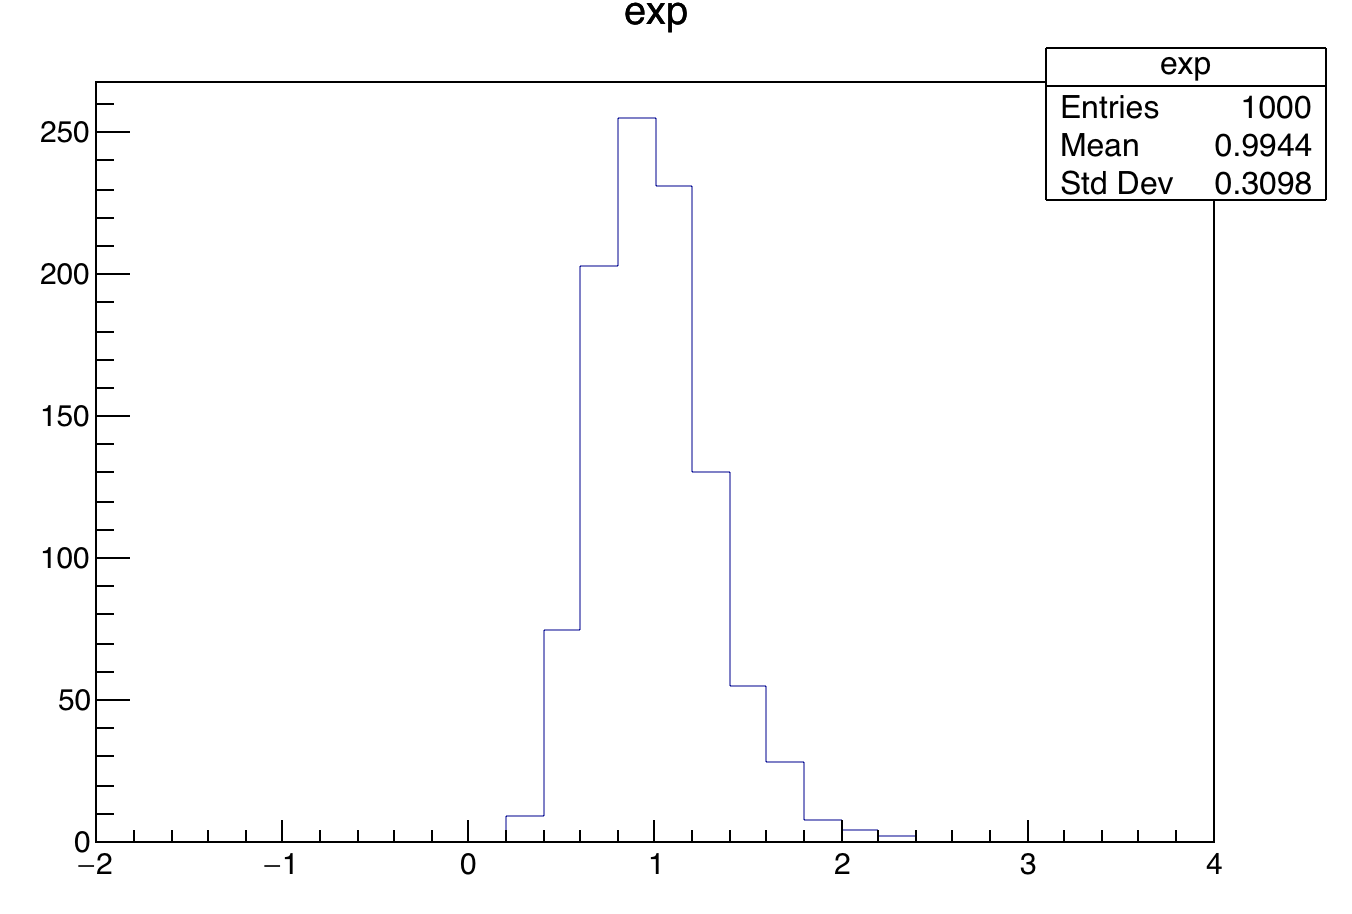
\includegraphics[scale=0.5]{exp}
\caption{tau distribution}
\label{fig:label}
\end{figure}\\
 (b)
 We can get the maximum likelihood function:
 \begin{equation}
 L=\prod_{i=1}^n\lambda e^{-\lambda t_i}
 \end{equation}
 we use $ \frac{\partial logL}{\partial \lambda}=0$ : 
 \begin{equation}
 \lambda=\frac{n}{\sum t_i}
 \end{equation}
\begin{figure}[htb]
\centering
\subfloat[n=5]{%
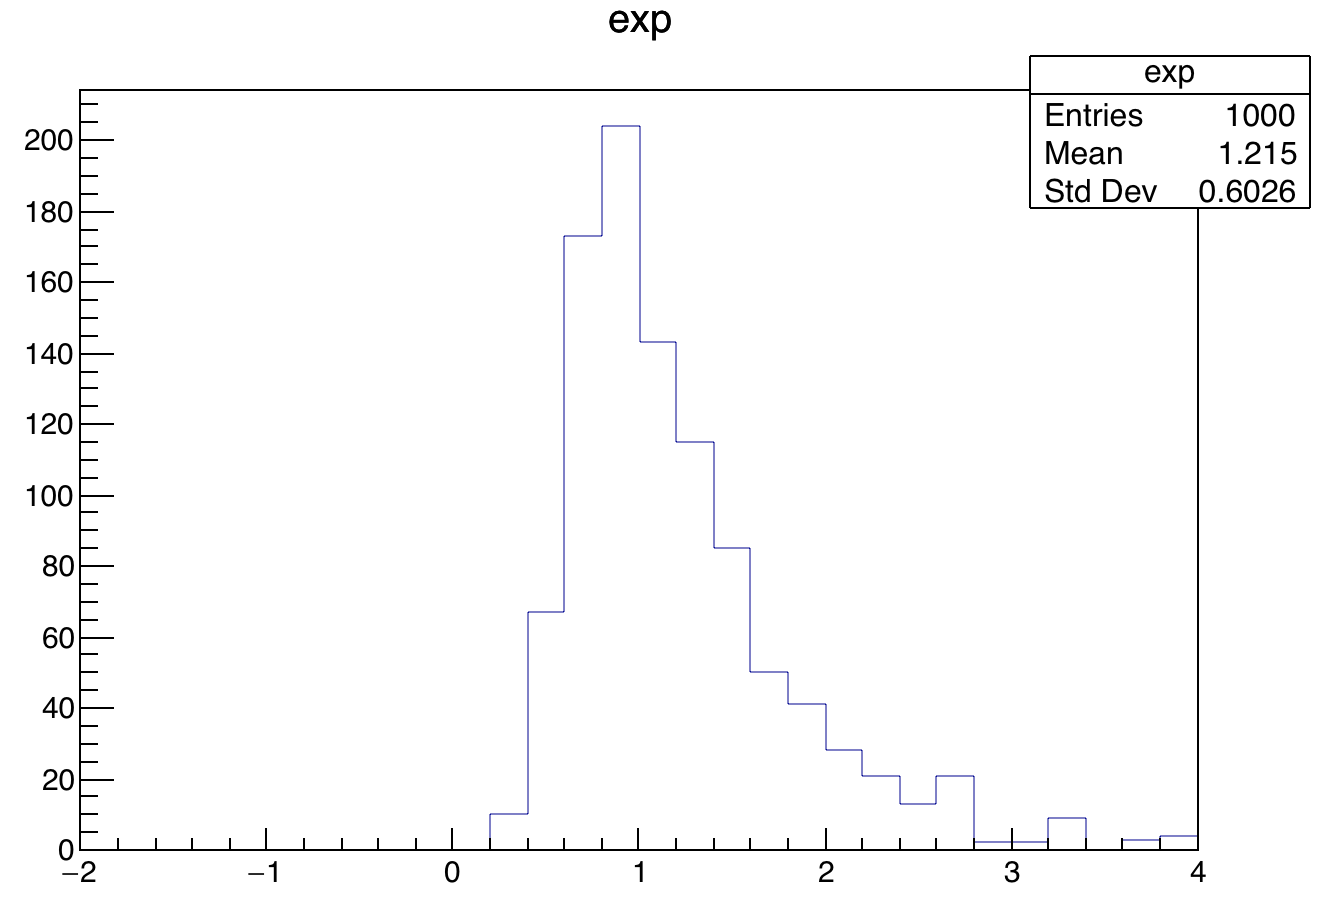
\includegraphics[width=.24\textwidth]{n=5}}\hfill
\subfloat[n=10]{%
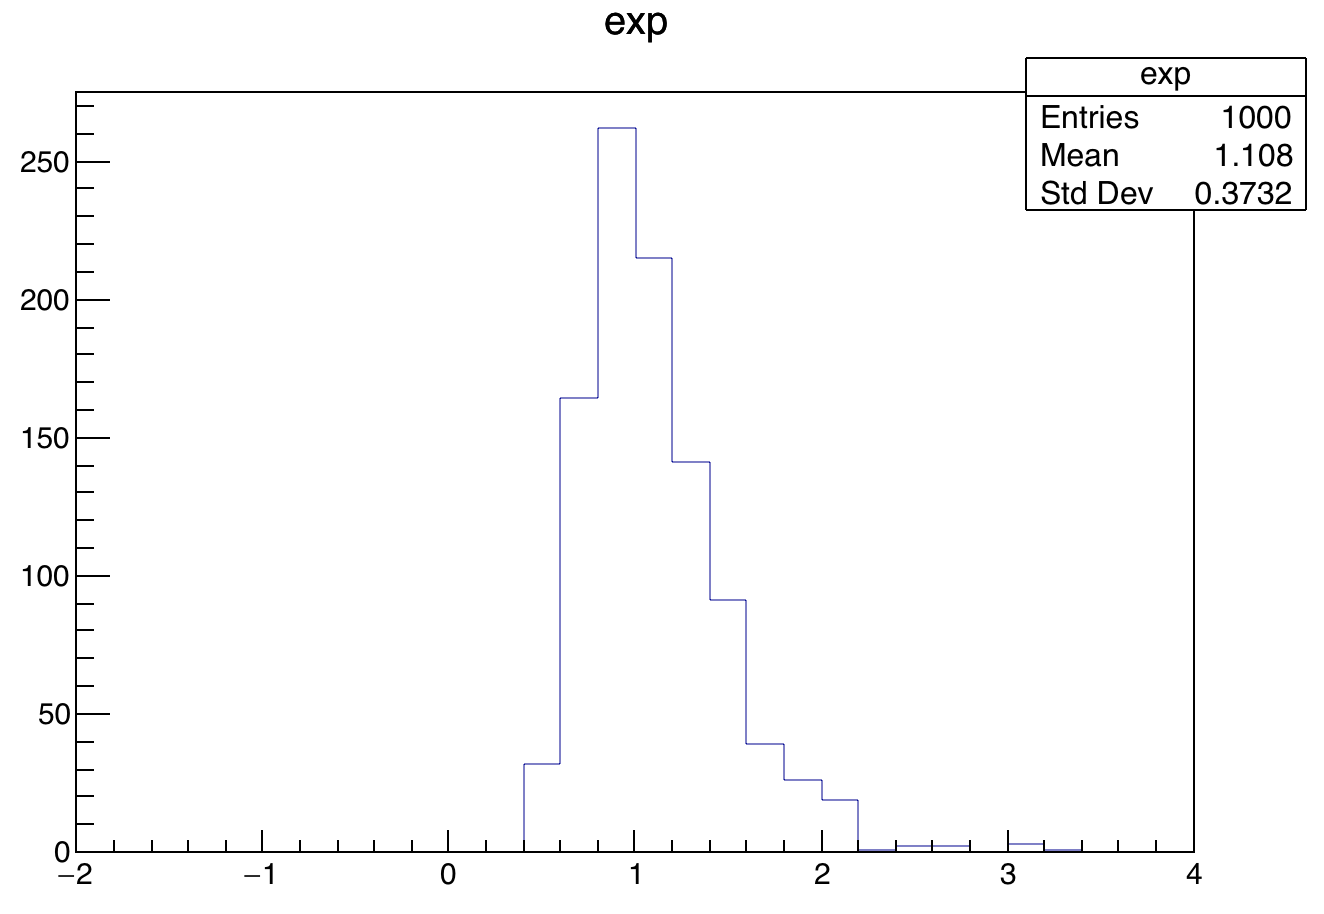
\includegraphics[width=.24\textwidth]{n=10}}\hfill
\subfloat[n=100]{%
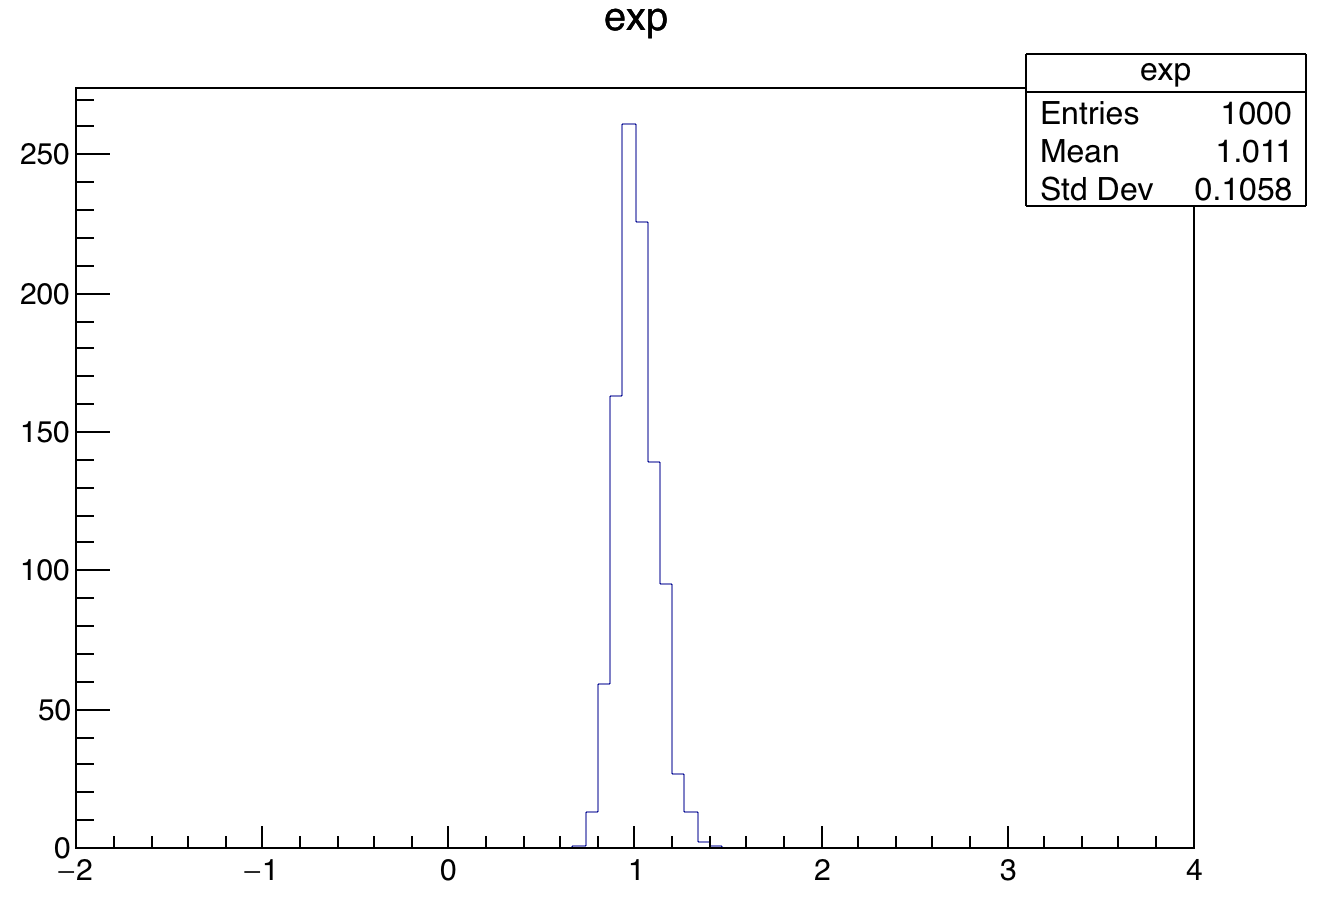
\includegraphics[width=.24\textwidth]{n=100}}\hfill
\caption{lambda distribution}
\label{fig:1}
\end{figure}


 
 \section{6.8}
 (a)
 The maximum likelihood function is : 
 \begin{equation}
 L=\frac{1}{N^N}
 \end{equation}
 When $N=1$, the L is maximum.It is wrong.
 (b)
 We can take the $n_{max}$ as the $\hat{N}_{taxi}$.
 \begin{equation}
 \begin{aligned}
 E[\hat{N}_{taxi}]&=\sum_{i=N}^{N_{taxi}}\frac{iC_{i-1}^{N-1}}{C_{N_{taxi}}^N}\\
 &=\sum_{i=N}^{N_{taxi}}N\frac{C_{i}^{N}}{C_{N_{taxi}}^N}\\
 &=\frac{N(N_{taxi}+1)}{N+1}
 \end{aligned}
 \end{equation}
 
 \begin{equation}
 \begin{aligned}
E[\hat{N}_{taxi}^2]&=\sum_{i=N}^{N_{taxi}}\frac{i^2C_{i-1}^{N-1}}{C_{N_{taxi}}^N}\\
&=\sum_{i=N}^{N_{taxi}}N\frac{(i+1)C_{i}^{N}-C_{i}^{N}}{C_{N_{taxi}}^N}\\
&=\sum_{i=N}^{N_{taxi}}N\frac{(N+1)C_{i+1}^{N+1}-C_{i}^{N}}{C_{N_{taxi}}^N}\\
&=N(N+1)\frac{C^{N+2}_{N_{taxi}+2}}{C_{N_{taxi}}^N}-N\frac{C^{N+1}_{N_{taxi}+1}}{C_{N_{taxi}}^N}
 \end{aligned}
 \end{equation}
 
 So we can get the variant:
 \begin{equation}
 V[\hat{N}_{taxi}]=\frac{(N_{taxi}+1)(N_{taxi}-N)N}{(N+2)(N+1)^2}
 \end{equation}
 
 
 
 \section{6.9}
 
 The maximum likelihood function is :
 \begin{equation}
 L=\prod_{i=1}^N\frac{(\theta a(x_i))^{n_i}}{n!}e^{-\theta a(x_i)}
 \end{equation}
 We use $\frac{\partial logL}{\partial \theta}=0$
 \begin{equation}
 \hat{\theta}=\frac{\sum_{i=1}^Nn_i}{\sum_{i=1}^Na(x_i)}
 \end{equation}
 
  \begin{equation}
 E[\hat{\theta}]=\frac{\sum_{i=1}^N\theta a(x_i)}{\sum_{i=1}^Na(x_i)}=\theta
 \end{equation}

  \begin{equation}
 V[\hat{\theta}]=\frac{\sum_{i=1}^NV[n_i]}{(\sum_{i=1}^Na(x_i))^2}=\frac{\theta}{\sum_{i=1}^Na(x_i)}
 \end{equation}
 
 and the minimum border of variant is :
 \begin{equation}
 V[\hat{\theta}]>\frac{1}{E[-\frac{\partial^2logL}{\partial\theta^2}]}=\frac{1}{\sum_{i=1}^NE[\frac{n_i}{\theta^2}]}=\frac{\theta}{\sum_{i=1}^Na(x_i)}
 \end{equation}
 
 \section{6.10}
 According to the 6.9 :
 \begin{equation}
 \begin{aligned}
 \hat{\theta}_{\nu}=\frac{\sum_{i=1}^Nn_i}{\sum_{i=1}^NE_i\epsilon(E_i)L_i}\\
 \hat{\theta}_{\bar{\nu}}=\frac{\sum_{i=1}^N\bar{n_i}}{\sum_{i=1}^NE_i\epsilon(E_i)L_i}\\
 \end{aligned}
 \end{equation}
 So we can solve:
  \begin{equation}
 \begin{aligned}
 \left\langle q \right\rangle=\frac{3\pi}{8G^2M}(3\theta_{\nu}-\theta_{\bar{\nu}})\\
 \left\langle \bar{q} \right\rangle=\frac{3\pi}{8G^2M}(3\theta_{\bar{\nu}}-\theta_{\nu})\\
 \end{aligned}
 \end{equation}
 So 
 \begin{equation}
  \left\langle \hat{g} \right\rangle=1-\frac{6\pi}{8G^2M\sum_{i=1}^NE_i\epsilon(E_i)L_i}[\sum_{i=1}^N(n_i+\bar{n}_i)]
 \end{equation}
 
 
 \section{6.11}
 
 
 
 
 
 
 
 
 
 
 
 
 
 
 
\end{CJK*}
\end{document}
